\documentclass[12pt,a4paper]{report}
\usepackage{graphicx}
\usepackage{fancyhdr}
\usepackage{lastpage}
\usepackage{titlesec}
\usepackage{tabularx}
\usepackage{xcolor,colortbl}
\usepackage{multirow}
\usepackage[sfdefault]{roboto}
\usepackage[T1]{fontenc}
\usepackage{subfig}
\usepackage{wrapfig,lipsum,booktabs}

\usepackage{geometry}
% \geometry{
%  a4paper,
%  left=35mm,
%  top=35mm,
%  }

\newcommand{\splitlayout}[2]{
	\begin{minipage}{0.6\textwidth}
		#1
	\end{minipage}
	\hfill
	\begin{minipage}{0.35\textwidth}
		#2
	\end{minipage}	
}

\setlength{\parindent}{0pt}
\bibliographystyle{plain}


\definecolor{LightCyan}{rgb}{0.88,1,1}
\definecolor{Gray}{gray}{0.85}

\newcommand*{\IhrVorname}{Lukas}
\newcommand*{\IhrNachname}{Kreussel}
\newcommand*{\IhreArbeit}{Comparison of Deep-Image-Embedding Methods }

\pagestyle{fancy}
\fancyhf{}
\rhead{\IhrVorname\space\IhrNachname}
\lhead{\IhreArbeit}
\cfoot{\thepage}

\begin{document}
\begin{titlepage}
	\centering
	{\scshape\LARGE Ostbayerische Technische Hochschule Amberg-Weiden\par}
	\vspace{1cm}
	{\scshape\Large Deep Vision\par}
	\vspace{1.5cm}
    \title{\IhreArbeit}
	{\huge\bfseries \IhreArbeit \par}
	\vspace{2cm}
	{\Large\itshape \IhrVorname \space \IhrNachname \par}

	\vfill

	{\large \today\par}
\end{titlepage}

\newpage
\tableofcontents
\newpage
\chapter{Introduction}

Deep image embeddings are a type of feature representation of images that can be used for a variety of tasks.
The main advantage of using deep image embeddings over traditional hand-crafted features is that they can be learned directly from data.
This means that they can be automatically generated from a large dataset, which can be beneficial when training data is limited.


There are many different ways to generate deep image embeddings, but one of the most popular methods is to use a convolutional neural network (CNN).
Another popular method, especially in recent years, is to use vision transformer networks (ViT).
These networks are trained to embed an image into a vector representation.
Most loss-metrics try to minimize the distance between the embedding vectors of similar images and maximize the distance of different images.	

Deep image embeddings can be used for image retrieval, object detection, and image classification.
In image retrieval, deep image embeddings can be used to represent images in a low-dimensional space.
This makes it possible to search for similar images by using a similarity metric such as Euclidean distance.
In object detection, deep image embeddings can be used to represent images at different resolutions.
This is helpful because the object of interest may be located at different positions in the image depending on the resolution.
In image classification, deep image embeddings can be used to represent images in a high-dimensional space.
This makes it possible to use a classifier such as a support vector machine (SVM) to learn a decision boundary that can be used to classify images.

\newpage
\chapter{Materials}

\section{Datasets}

\subsubsection{Tiny Imagenet}
The  \textit{Tiny ImageNet} dataset is a subset of the ImageNet dataset.
It contains only only colored images with 64x64 pixels per image and was created as an alternative to the CIFAR \cite{cifar} datasets.
The dataset contains 200 different classes with a total of 500 images per class.\cite{tinyimagenet}
A subset of 50 classes is used in the experiments to test different backbones, loss functions and embedding sizes.

\begin{figure}[h]
    \centering
    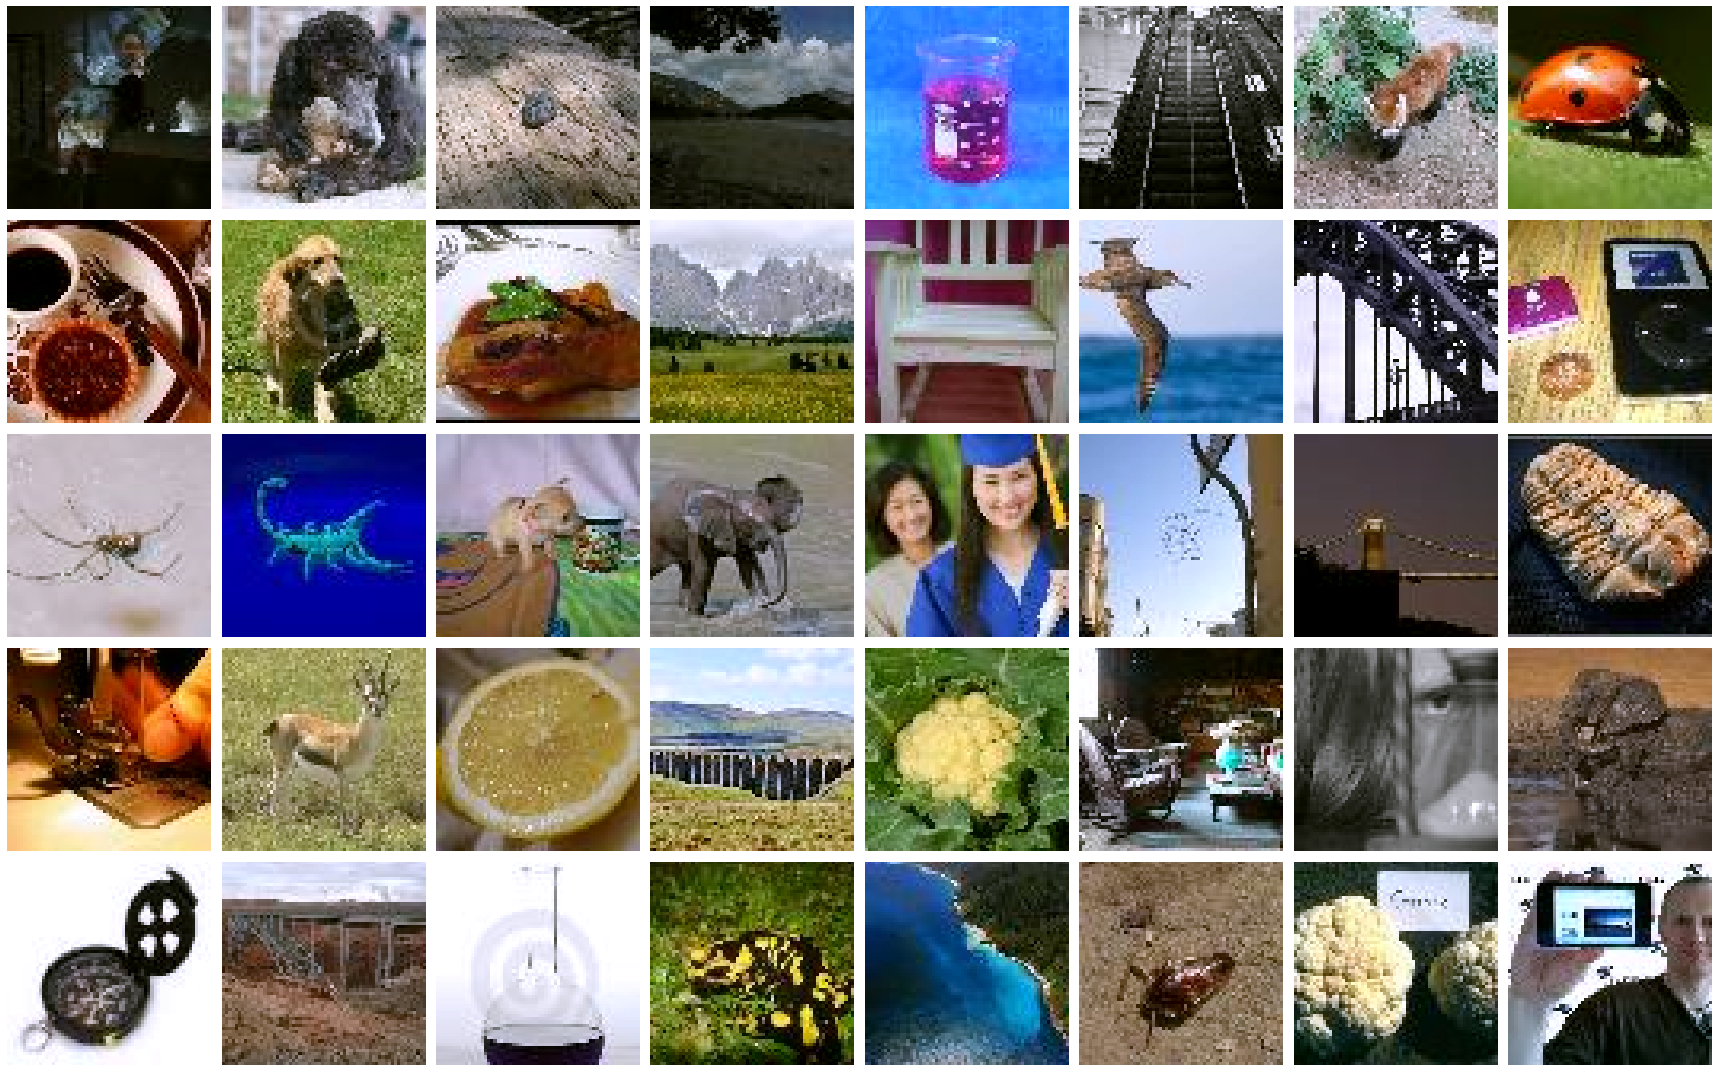
\includegraphics[width=0.9\textwidth]{./images/tinyimagenet.png}
	\caption{Tiny Imagenet}
\end{figure}

\newpage

\subsubsection{Internal and External Parts of Cars}
The \textit{Internal and External Parts of Cars} dataset \cite{internalexternal} is a subset of the CompCars \cite{carparts} dataset.
It contains images of different internal and external car parts.
In total there are 27.618 images from 8 different classes.
The dataset is used in the experiments to test zero-shot classification performance and a subset of 20 images per class is used to measure the performance on very small datasets.

\begin{figure}[h]
    \centering
    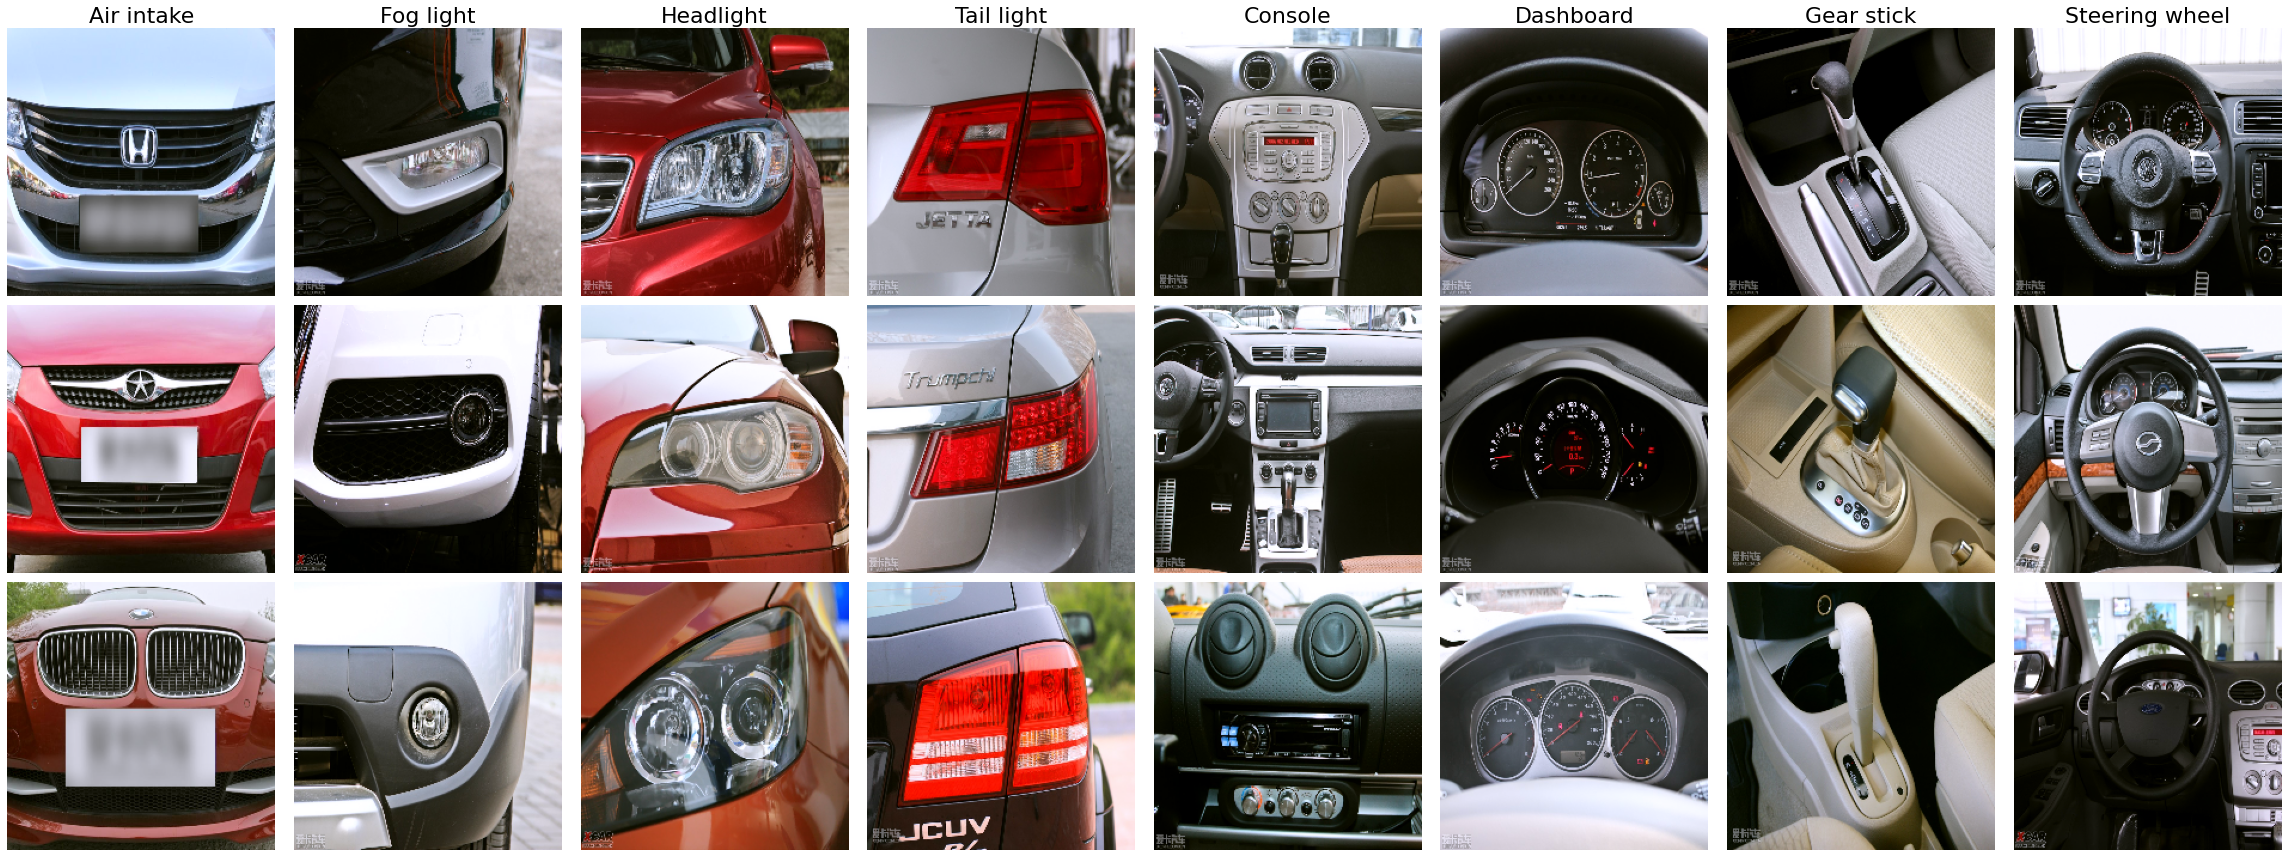
\includegraphics[width=\textwidth]{./images/carparst.png}
	\caption{Internal and External Parts of Cars}
\end{figure}


\newpage


\chapter{Methods}
\section{Image embedding networks}


An image embedding network is a neural network that is trained to map images into a lower-dimensional space while retaining as much information about the original image as possible.
This is done by learning to find relationships between the pixels in the image.
The default architecture for this task is a backbone network that is trained to extract the features of an image (e.g. any CNN) followed by a multi-layer-perceptron (MLP) that compresses the features into a one dimensional vector.  

\begin{figure}[h]
    \centering
	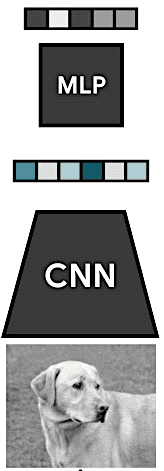
\includegraphics[height=4cm]{./images/embedding_network.png}
	\caption{Default image embedding network}
\end{figure}

\newpage

\section{Siamese networks}
A Siamese neural network is a neural network that consists of two or more identical networks.\cite{signatureVerification}
To train a network to generate deep image embeddings from images, these multiple networks are commonly used in the training step,
where the embeddings are calculated for each image and a loss function is used to minimize or maximize the distance between the embeddings,
depending on the task. For inference only on of the networks is used.

\begin{figure}[h]
    \centering
    \subfloat[\centering Positives]{{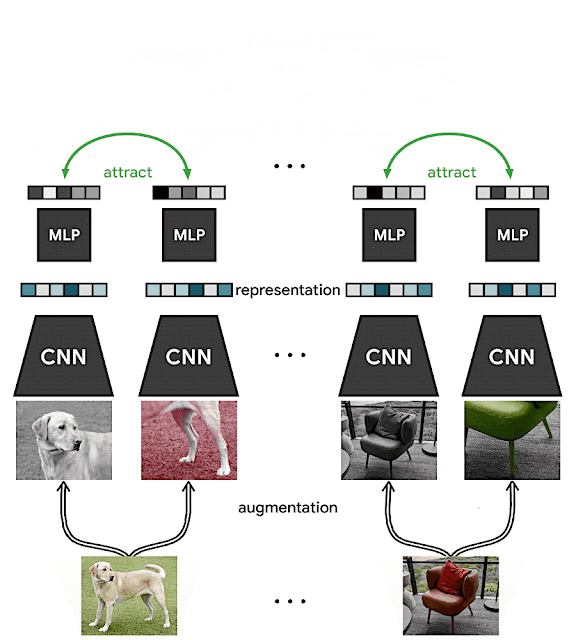
\includegraphics[width=5cm]{./images/siamese_attract.png} }}
    \qquad
    \subfloat[\centering Negatives]{{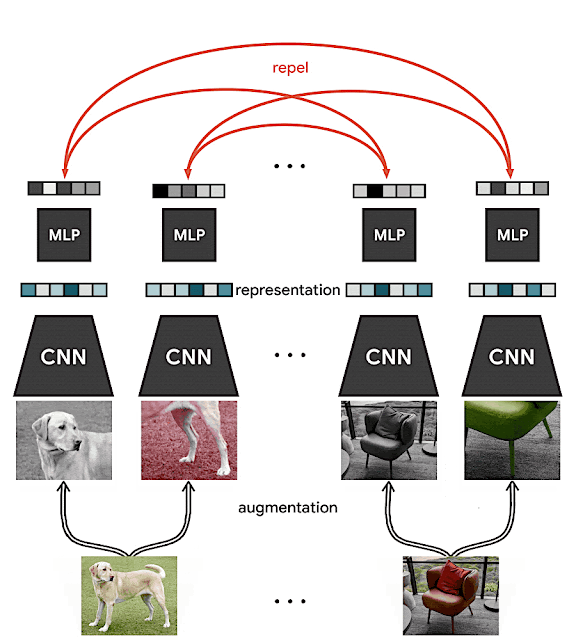
\includegraphics[width=5cm]{./images/siamese_repel.png} }}
    \caption{Similarity Training in Siamese Networks \cite{simclrartikle}}
\end{figure}

Frameworks like SimCLR\cite{simclr} don't use multiple networks for training, but instead use a single network that processes every image in a mini batch.
The resulting embeddings are then sorted by labels and grouped into positives and negatives.
Then a loss function is used to minimize distance between the positives and maximize the distance between the negatives.
This approach is a lot faster and uses less memory than using multiple networks.
\\
There is also the \textit{PyTorch Metric Learning}\cite{musgrave2020pytorch} library available for this task, that implements the same approach for generic pytorch models.

\newpage

\section{Backbones}
For the feature extraction two different network architectures were used.
CNN which use the principle of convolutions and transformers which use the principle of local and global attention to extract information from images. 
The following Backbones were used:
\begin{itemize}
	\item CNNs:\begin{itemize}
		\item \textbf{ResNet 50} \cite{resnet}
		\item \textbf{EfficientNetV2} \cite{EfficientNetV2}
		\item \textbf{MobilNetV3} \cite{MobilNetV3}
		\item \textbf{DenseNet} \cite{DenseNet}
	\end{itemize}
	\item Transformers:\begin{itemize}
		\item \textbf{Vit} \cite{ViT}
		\item \textbf{Swin} \cite{liu2021swin}
    \end{itemize}
\end{itemize}

\section{Losses}
The KNN-classification in the experiments assumes the embeddings for similar images to have a small distance to each other
and a large distance to the embeddings of different images.
To achieve this contrastive loss functions are used.
The most basic contrastive loss function can be described as the distance between the embeddings of two images if they are positives and a margin (any number e.g. 4) minus the distance of the embeddings if the images are negatives.
More advanced contrastive loss functions (e.g. SupConLoss) build groups of embeddings by a given label and try to minimize the distance within each group and maximize the distance between the different groups of a batch.
Another option is to use different distance metrics like cosine distance, euclidean distance, etc.
\\
The following loss functions were used:
\begin{itemize}
	\item \textbf{ContrastiveLoss} \cite{ContrastiveLoss}
 	\item \textbf{TripletLoss} \cite{TripletLoss}
  	\item \textbf{SupConLoss} \cite{SupConLoss}
    \item \textbf{SNRLoss} \cite{SNRLoss}
    \item \textbf{NTXentLoss} \cite{simclr}
\end{itemize}

\section{Augmentation techniques}
Image augmentation is the process of taking an image and applying random transformations to the image to produce a new image.
The random transformations can be things like Flip, Crop, Rotate, and Warp.
These transformations help to improve the ability of the model to generalize to new data by increasing the amount of data that the model sees.
They are especially useful for small datasets where the model is not able to generalize to new data.
The following augmentation techniques describe modules that automatically augment images:
\begin{itemize}
	\item \textbf{AutoAugment} \cite{AutoAugment}
 	\item \textbf{RandAugment} \cite{RandAugment}
  	\item \textbf{TrivialAugment} \cite{TrivialAugmentWide}
\end{itemize}

\section{KNN search}
K-nearest-neighbor(KNN) search is a method of pattern recognition where an unknown pattern is classified by its similarity to known patterns.
The KNN algorithm groups data points together based on their distance from a given point, called a query point.
The query point is then assigned the class label of the most common class among its K neighbors.
The KNN algorithm can be used to perform classification tasks on image embeddings.


\begin{figure}[h]
    \centering
    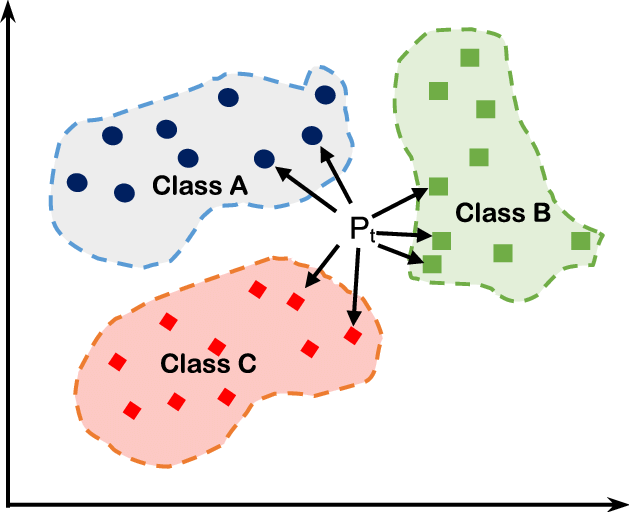
\includegraphics[width=0.5\textwidth]{./images/knn.png}
	\caption{KNN search}
\end{figure}

\newpage

\section{t-SNE}
T-distributed stochastic neighbor embedding (t-SNE) is a statistic method for embedding visualization.
It is a technique for dimensionality reduction that is particularly well suited for the visualization of high-dimensional data.
The algorithm is based on the idea of finding a low-dimensional representation of the data that preserves the local structure of the data.

\begin{figure}[h]
    \centering
    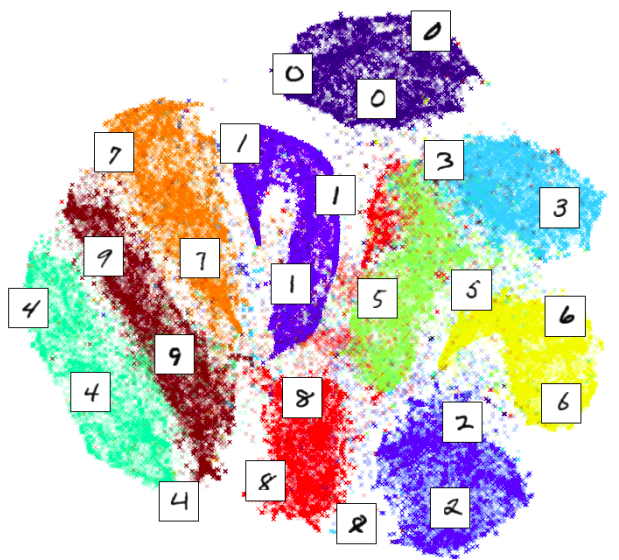
\includegraphics[width=0.5\textwidth]{./images/tsne-mnist.png}
	\caption{t-SNE visualization of MNIST}
\end{figure}

\chapter{Results and Discussion}

\newpage

\section{Backbone performance}
In this experiment different backbones were used to train a siamese network for five epochs on a subset of 50 classes of the Tiny ImageNet dataset.
No augmentations were used.
Each network had a target embedding size of 256, used the TripletLoss metric and was initialized with pretrained ImageNet weights.

\subsubsection{Results}

\splitlayout{
	Although ViT and Swin are a lot slower and need more memory than the other backbones they perform a lot better.
	This property can also be observed in NLP tasks, where transformers originated from.
	Small models like MobilNetV3 and EfficientNet seem to struggle to generate good embeddings for all classes.
	They would probably perform a lot better if the embedding tasks contains less classes.
	The ResNet50 baseline generates good embeddings and even outperforms the larger DenseNet169 backbone.
}{
	\begin{tabular}{ | c | c | }
		\hline
		Backbone & F1-Score \\ 
		\hline
		ResNet50 & 0.664 \\ 
		\hline
		EfficientNetV2 L & 0.540 \\ 
		\hline
		MobilNetV3 & 0.367 \\ 
		\hline
		DenseNet169 & 0.612 \\ 
		\hline
		ViT & 0.893 \\ 
		\hline
		Swin & 0.934 \\ 
		\hline
	\end{tabular}
}

\begin{figure}[h]
	\centering
	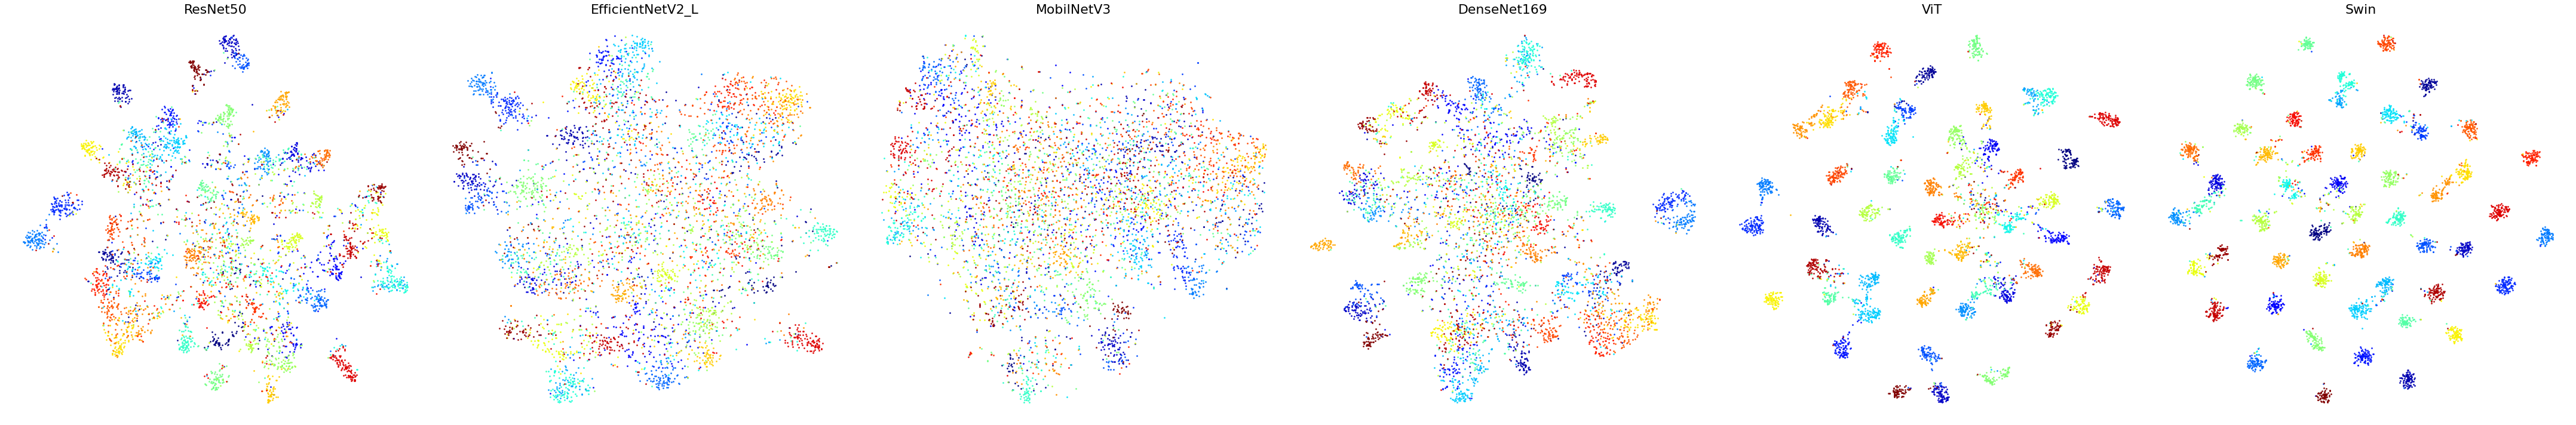
\includegraphics[width=0.9\textwidth]{../plots/backbones.png}
	\caption{t-SNE visualization of backbones}
\end{figure}

\newpage

\section{Significance of Loss Functions}

In this experiment different loss functions were used to train a siamese network for five epochs on a subset of 50 classes of the Tiny ImageNet dataset.
No augmentations were used.
As a backbone ResNet50 was used.
The network had a target embedding size of 256 and was initialized with pretrained ImageNet weights.


\subsubsection{Results}

\splitlayout{
	The SupConLoss function is the best performing loss function.
	It is also the only loss function that expects the data to be labeled and is optimized for supervised learning.
	The other loss functions are more general and can also be used for unsupervised learning.
	We trained the network with labeled data, so its expected that the SupConLoss function performs better than the other loss functions.
}{
	\begin{tabular}{ | c | c | }
		\hline
		Loss & F1-Score \\ 
		\hline
		ContrastiveLoss & 0.650 \\ 
		\hline
		TripletLoss & 0.660 \\ 
		\hline
		SupConLoss & 0.709 \\ 
		\hline
		SNRLoss & 0.685 \\ 
		\hline
		NTXentLoss & 0.618 \\ 
		\hline
	\end{tabular}
}

\begin{figure}[hb]
	\centering
	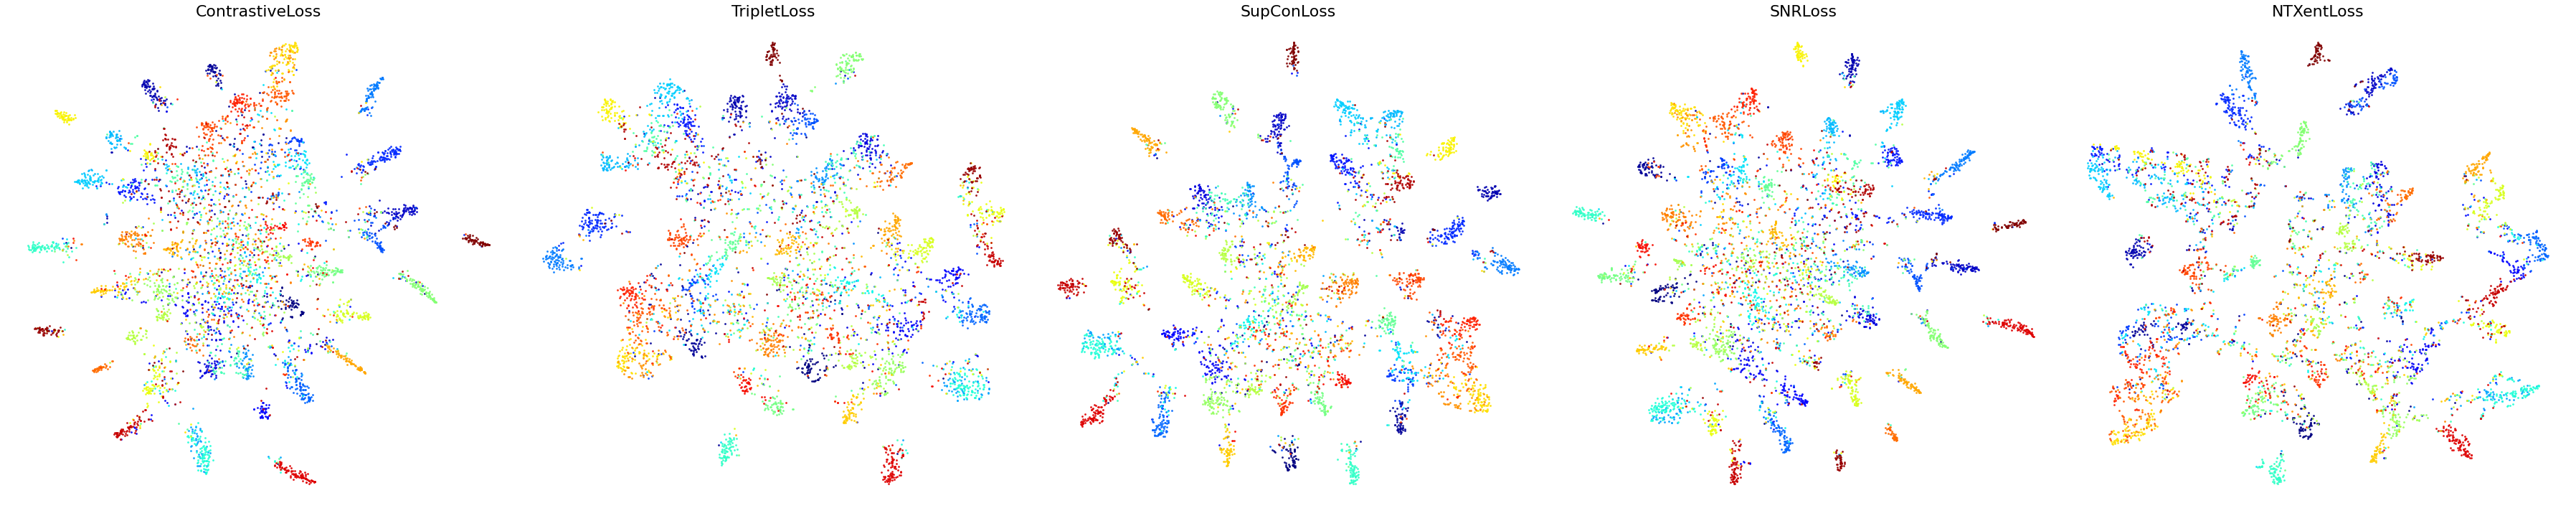
\includegraphics[width=0.9\textwidth]{../plots/losses.png}
	\caption{t-SNE visualization of loss functions}
\end{figure}

\newpage

\section{Differences in Embedding Sizes}

In this experiment different embedding sizes were used to train a siamese network for five epochs on a subset of 50 classes of the Tiny ImageNet dataset.
No augmentations were used.
As a backbone ResNet50 was used.
The network used the SupConLoss metric and was initialized with pretrained ImageNet weights.


\subsubsection{Results}
\splitlayout{
	The performance of the network get better with higher embedding sizes.
	This effect seams to plateau at an embedding sizes of 1024.
	With bigger embedding sizes the parameters of the model increase exponentially and we need a lot more calculations to perform KNN-Searches on the generated embeddings.
	So its not possible to scale the embedding size indefinitely.
}{
	\begin{tabular}{ | c | c | }
		\hline
		Embedding Size &  F1-Score \\ 
		\hline
		64 &  0.654 \\ 
		\hline
		128 & 0.683 \\ 
		\hline
		256 & 0.712 \\ 
		\hline
		512 & 0.719 \\ 
		\hline
		1024 & 0.724  \\ 
		\hline
		2048 & 0.731 \\ 
		\hline
	\end{tabular}
}

\begin{figure}[hb]
	\centering
	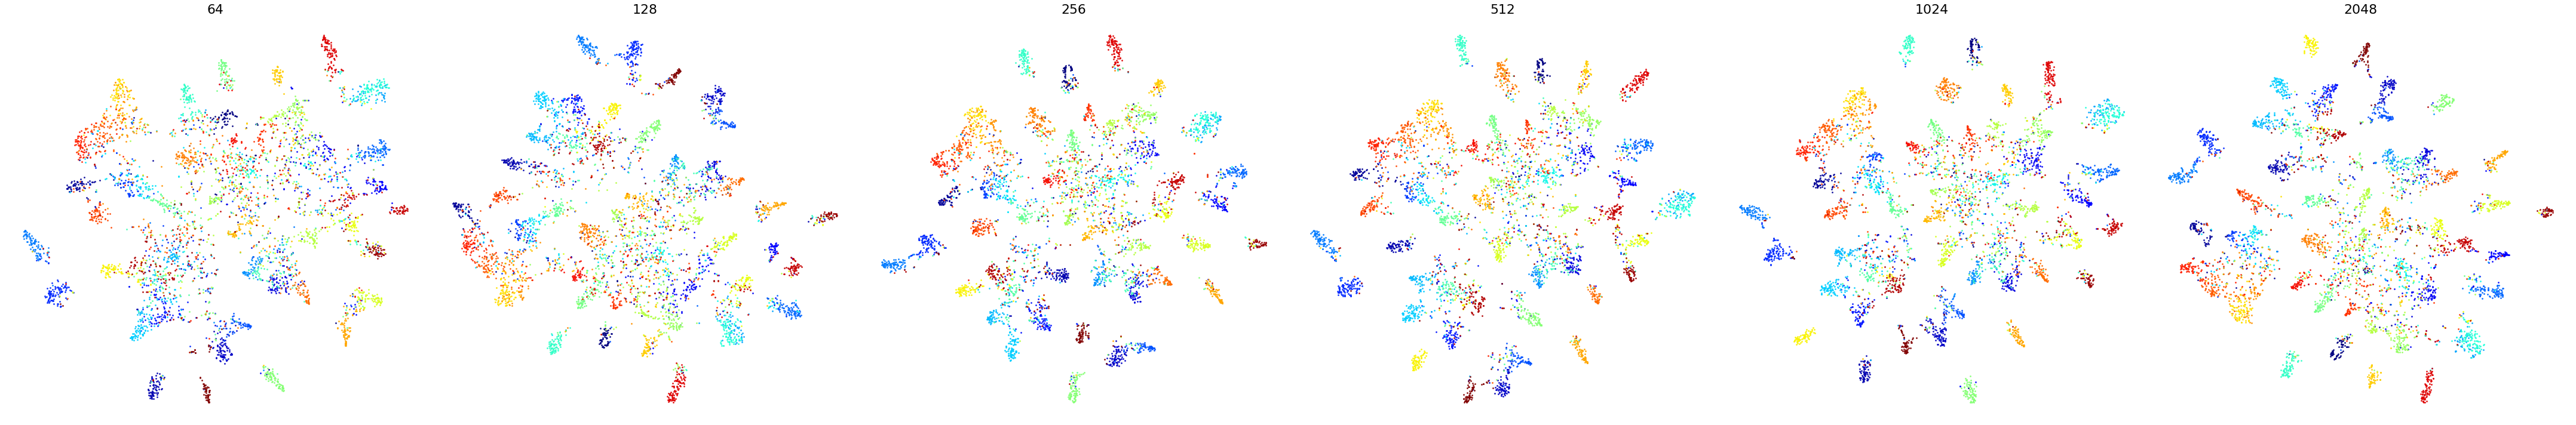
\includegraphics[width=0.9\textwidth]{../plots/embedding_size.png}
	\caption{t-SNE visualization of embedding sizes}
\end{figure}


\newpage


\section{Dependency on Dataset Size}

In this experiment different dataset with N samples per class were used to train a siamese network for five epochs on a subset of 50 classes of the Tiny ImageNet dataset.
For validation the same dataset as in the other experiments was used with 100 validation images for each of the classes.
No augmentations were used.
As a backbone ResNet50 was used.
The network used the SupConLoss metric and was initialized with pretrained ImageNet weights.


\subsubsection{Results}
\splitlayout{
	The performance of the network is extremely dependent on the size of the train dataset.
	Every network which was trained under the sample size of 200 can't generate usable embeddings.
	When trying to finetune a embedding network with very small sample sizes per class image augmentation methods should be used. 
}{
	\begin{tabular}{ | c | c | }
		\hline
		Samples per Class &  F1-Score \\ 
		\hline
		10 &  0.223 \\ 
		\hline
		20 & 0.280 \\ 
		\hline
		30 & 0.369 \\ 
		\hline
		50 & 0.443 \\ 
		\hline
		80 & 0.507  \\ 
		\hline
		100 & 0.520 \\ 
		\hline
		200 & 0.632 \\ 
		\hline
		400 & 0.703 \\ 
		\hline
	\end{tabular}
}

\begin{figure}[hb]
	\centering
	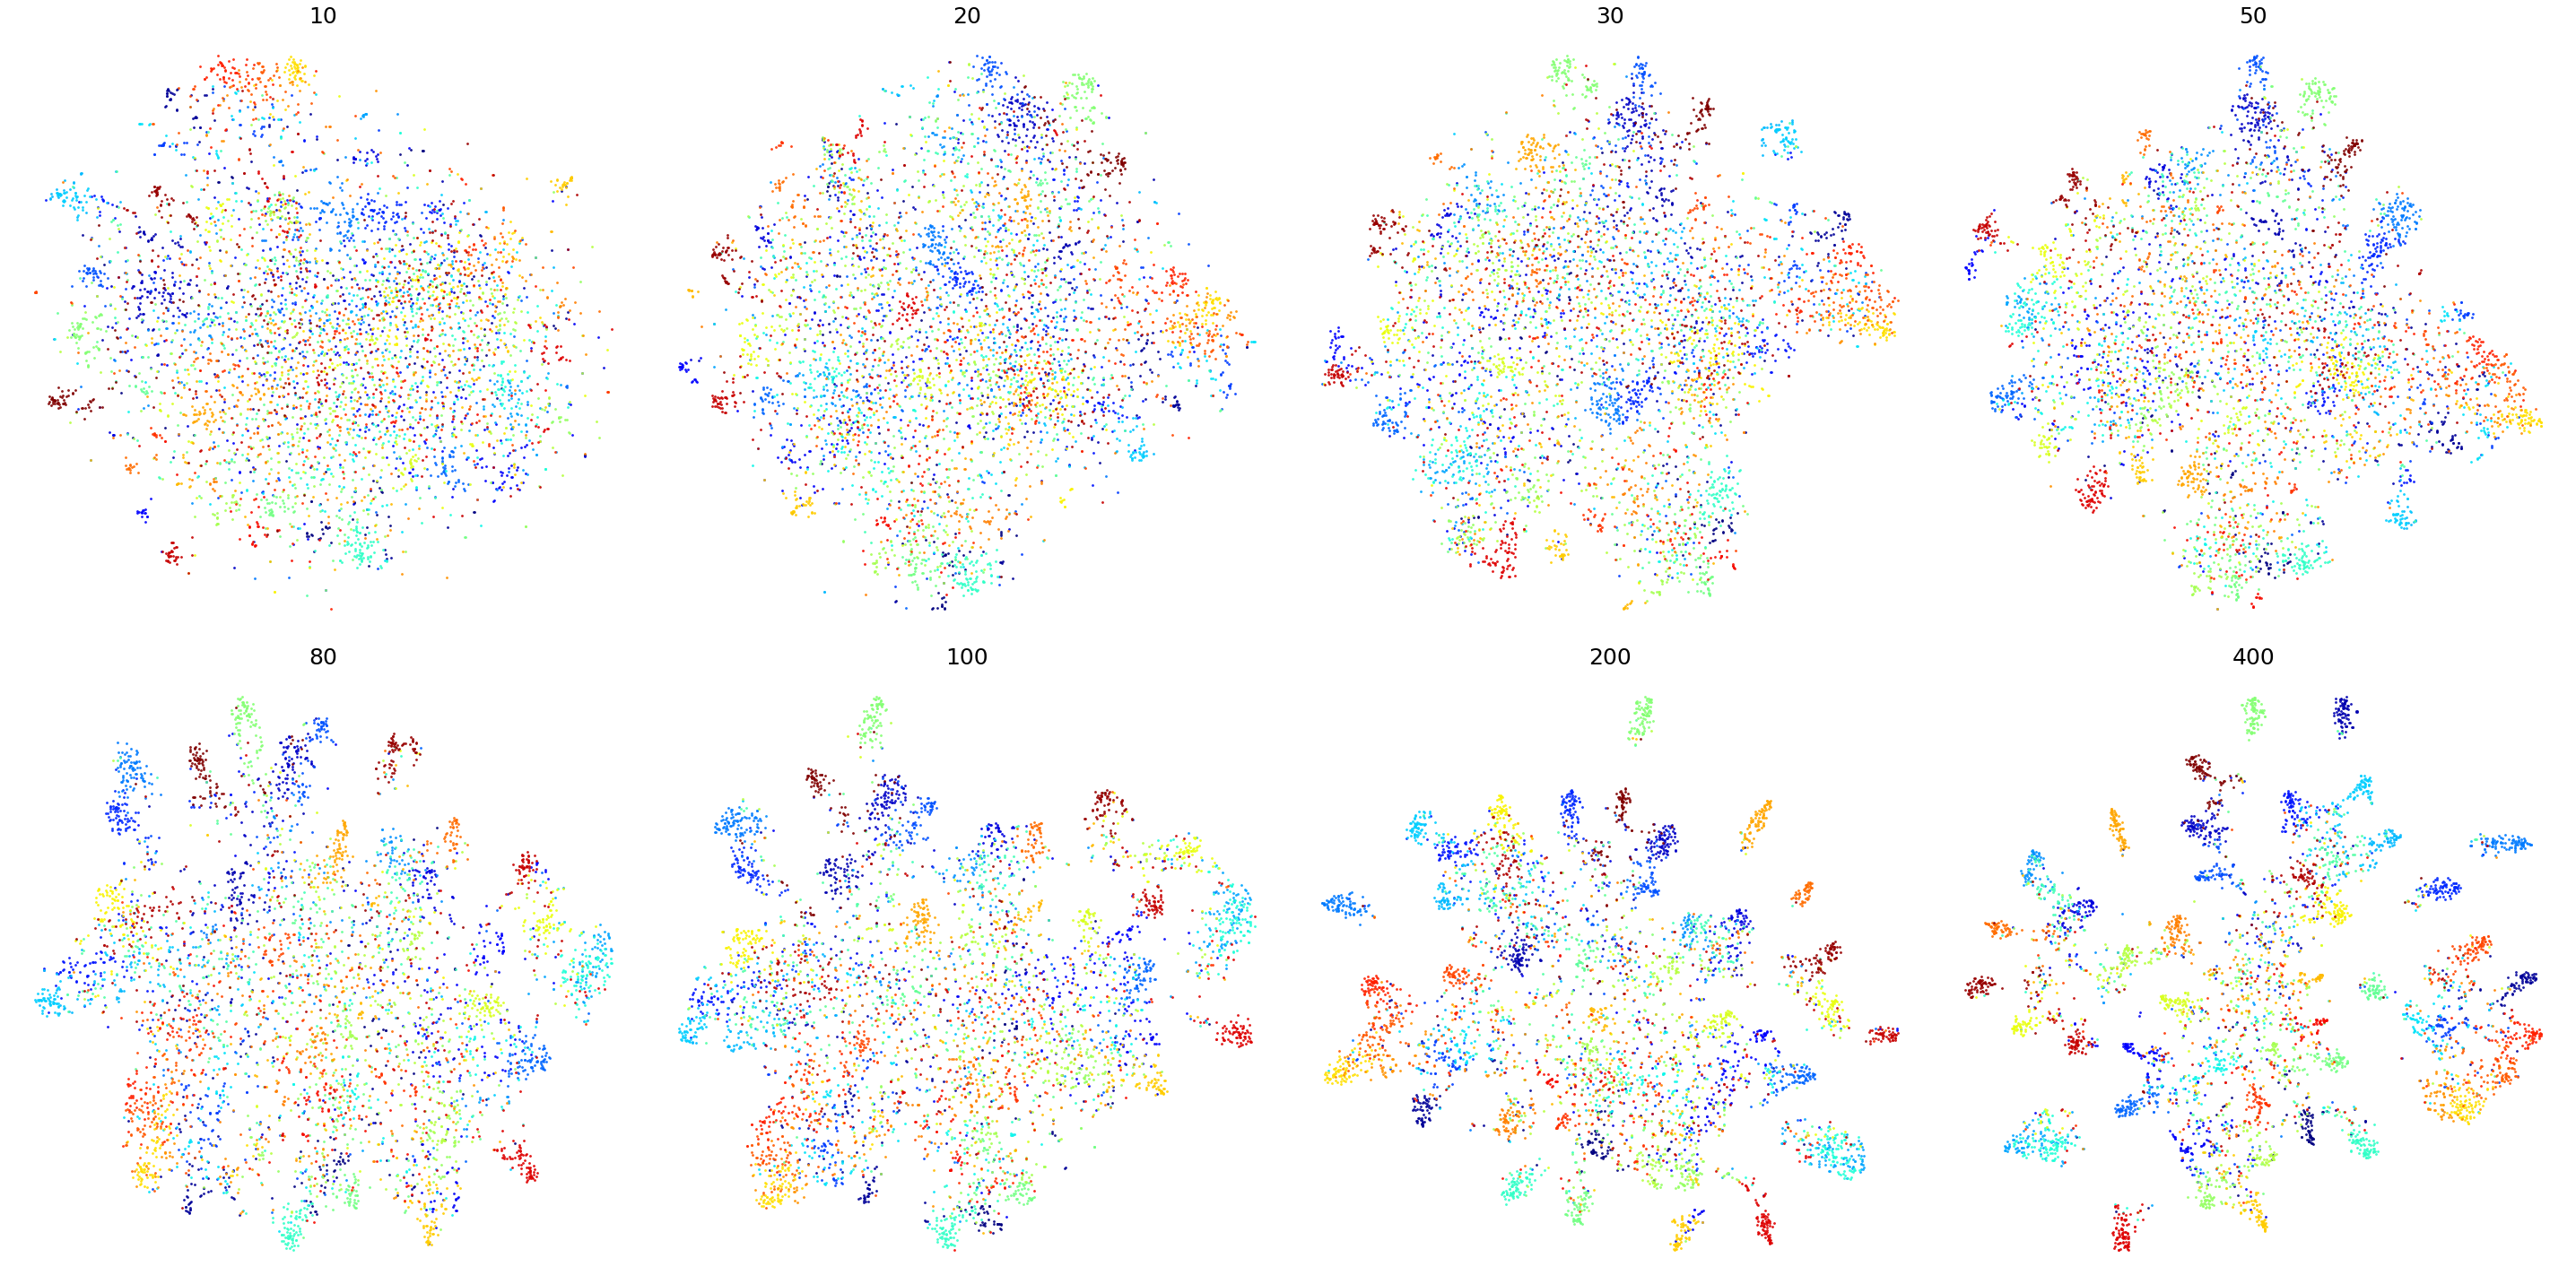
\includegraphics[width=0.9\textwidth]{../plots/dataset_size.png}
	\caption{t-SNE visualization of dataset sizes}
\end{figure}

\newpage

\section{Efficiency of augmentations}

In this experiment a dataset with 20 samples per class was build for 50 classes of the Tiny ImageNet dataset.
Then this dataset was augmented with the RandAugment module to N*20 samples per class.
For validation the same dataset as in the other experiments was used with 100 validation images for each of the classes.
As a backbone ResNet50 was used.
The network used the SupConLoss metric and was initialized with pretrained ImageNet weights.

\subsubsection{Results}
\splitlayout{
	Augmentations are a very effective way to boost the performance of the network and 
	to generalize the network,
	especially on a small dataset.
	Furthermore the performance seams to scale linearly with the number of augmentations.
	This is probably caused by the extremely small sample size per class.
	On bigger datasets the performance of the network is not affected that drastically by the number of augmentations.
}{
	\begin{tabular}{ | c | c | }
		\hline
		Factor &  F1-Score \\ 
		\hline
		1x (Baseline) &  0.306  \\ 
		\hline
		2x & 0.352 \\ 
		\hline
		4x & 0.437 \\ 
		\hline
		8x & 0.518 \\ 
		\hline
		16x & 0.569  \\ 
		\hline
	\end{tabular}
}

\begin{figure}[hb]
	\centering
	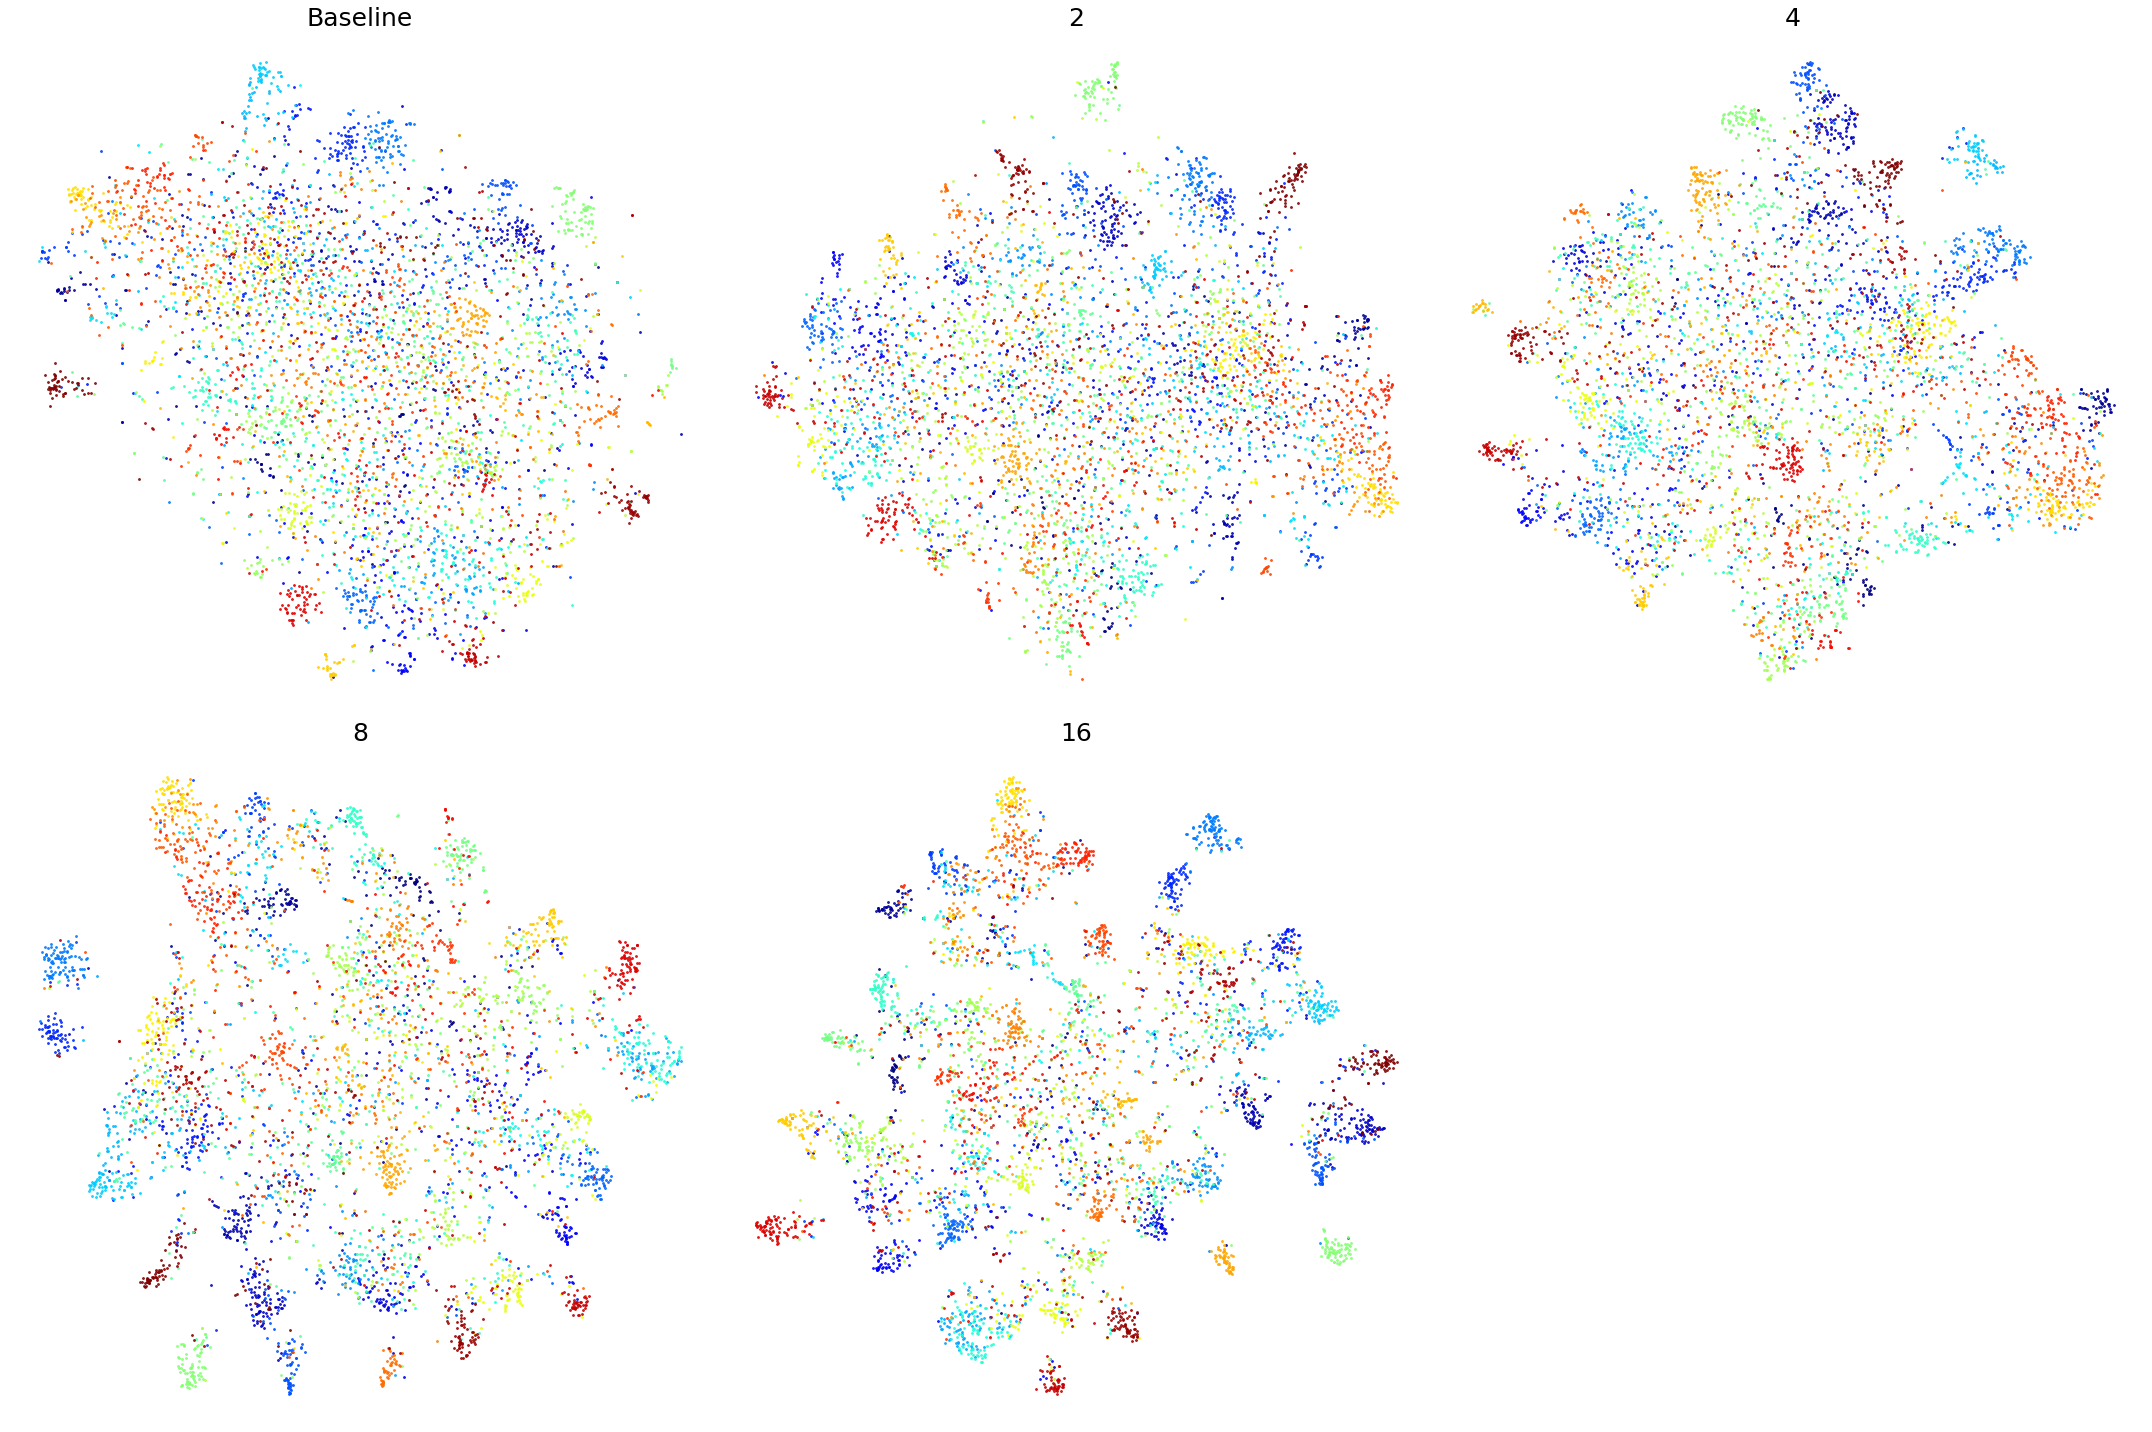
\includegraphics[width=0.9\textwidth]{../plots/augmentation_size.png}
	\caption{t-SNE visualization of augmentation factors}
\end{figure}

\newpage

\section{Testing different auto augmentation methods}
In this experiment a dataset with 20 samples per class was build for 50 classes of the Tiny ImageNet dataset.
Then this dataset was augmented with different auto augmentation modules by a factor of 4 to 80 samples per class.
For validation the same dataset as in the other experiments was used with 100 validation images for each of the classes.
As a backbone ResNet50 was used.
The network used the SupConLoss metric and was initialized with pretrained ImageNet weights.

\subsubsection{Results}
\splitlayout{
	RandAugment and TrivialAugment perform very similarly to each other.
	AutoAugment performs a bit worse than the other methodes.
	This is probably caused by the used imagenet augmentation profile, that is not suited for the Tiny ImageNet dataset.
	The other methodes dont depend on a profile that is finetuned on a dataset and can easily be applied to any dataset. 
}{
	\begin{tabular}{ | c | c | }
		\hline
		Method &  F1-Score \\ 
		\hline
		Baseline &  0.289  \\ 
		\hline
		AutoAugment & 0.392 \\ 
		\hline
		RandAugment & 0.436 \\ 
		\hline
		TrivialAugment & 0.441  \\ 
		\hline
	\end{tabular}
}

\begin{figure}[hb]
	\centering
	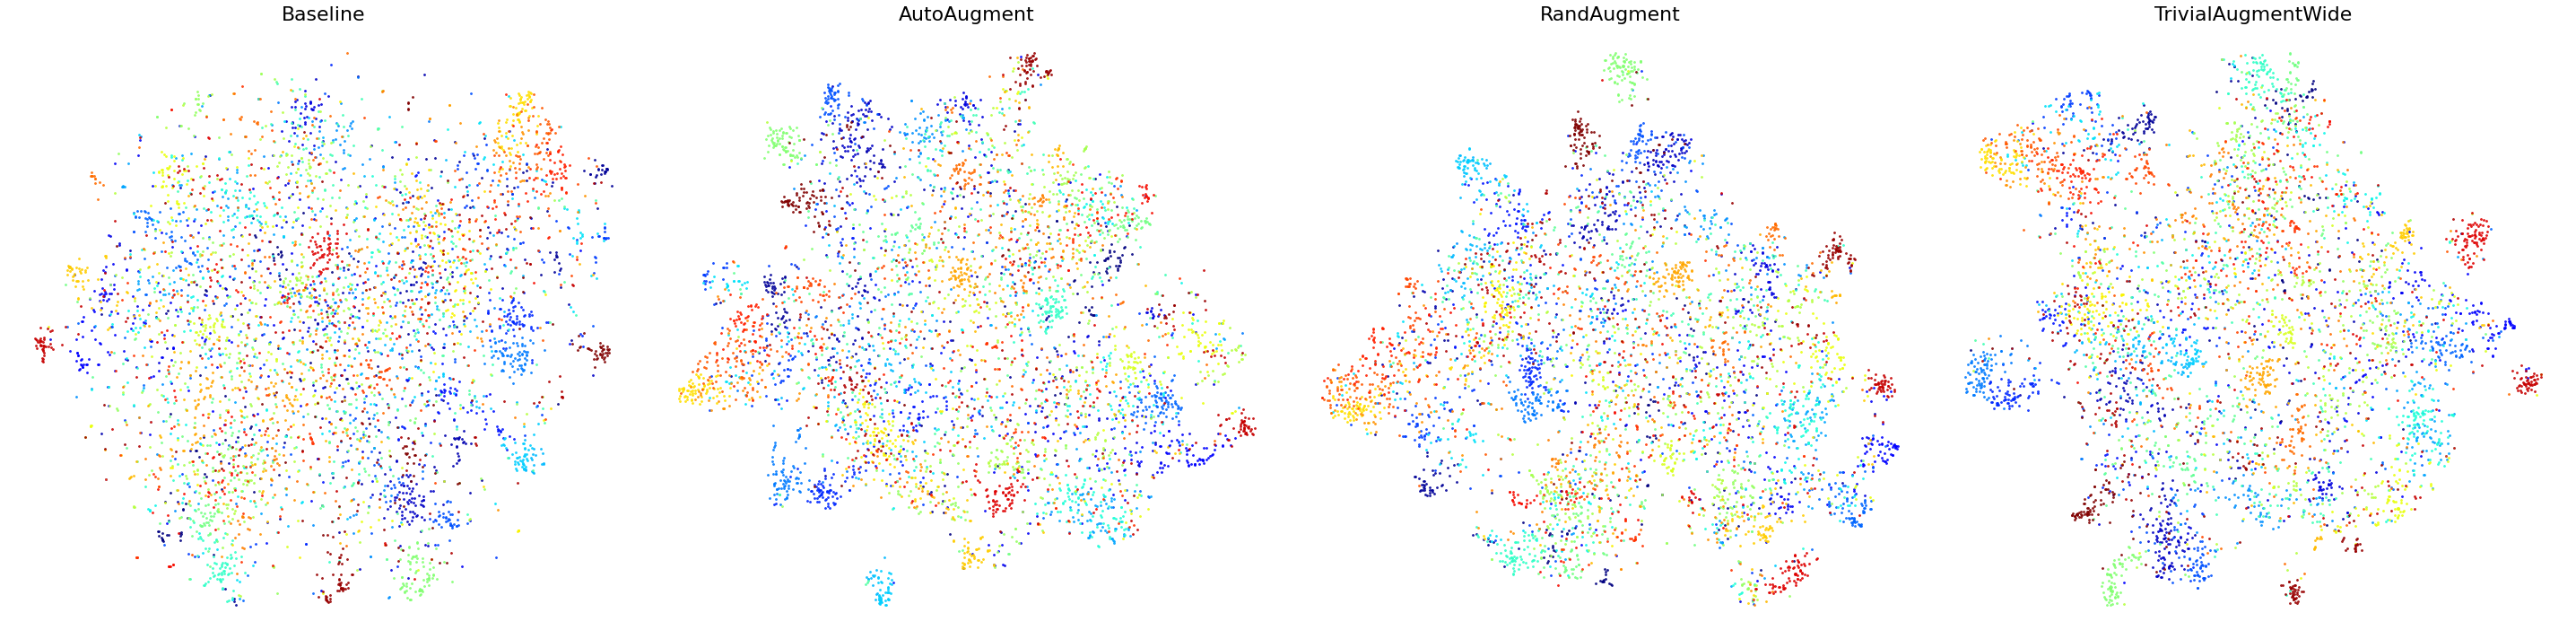
\includegraphics[width=0.9\textwidth]{../plots/augmentation_methods.png}
	\caption{t-SNE visualization of different augmentation methods}
\end{figure}

\newpage

\section{Testing zero shot capabilities}
In this experiment a SWIN model was finetuned on a four times augmented Tiny ImageNet dataset for 1 epoch.
Then the embeddings for 100 image per class of the "Internal and External Parts of Cars"-Dataset where calculated.
Half of these embeddings were used for the KNN search the other half was used to validate the model.

\subsubsection{Results}
\splitlayout{
The zero shot capabilities of embedding networks are very good.
Especially when a transformer based backbone is used.
This allows ambedding networks to be trained on a very broad dataset like ImageNet-22K and then be used in a detection task in a different domain without the need to finetune the network on this new task.

}{
	\begin{tabular}{ | c | }
		\hline
		F1-Score \\ 
		\hline
		0.865  \\ 
		\hline
	\end{tabular}
}

\begin{figure}[hb]
	\centering
	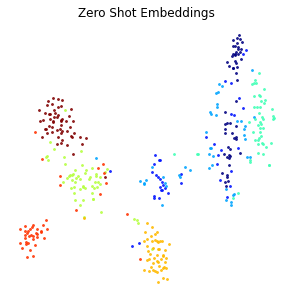
\includegraphics[width=0.4\textwidth]{../plots/zero_shot_embeddings.png}
	\caption{t-SNE visualization of zero shot embeddings}
\end{figure}

\newpage

\section{Combining the above observations}

In this experiment we try to train a model on 4 classes of the "Internal and External Parts of Cars"-dataset with 20 samples per class.
Then we validate the model against all 8 classes of the dataset with 230 validation images each.
As a backbone SWIN was used with a embedding size of 1024.
SupConLoss was used as a loss metric and the model was initialized with pretrained ImageNet weights.
The dataset was augmented by a factor of 16 with the RandAugment module.

\subsubsection{Results}
\splitlayout{
	By combining the observations of the above experiments we can create a model on a small dataset that can perform very well in a classification task.
	Furthermore the resulting model can create descriptive embeddings for unknown classes that reside in the same domain as the trained classes.
}{
	\begin{tabular}{ | c | c | }
		\hline
		Mode & F1-Score \\ 
		\hline
		Trained & 0.995  \\ 
		\hline
		Zero-Shot & 0.975  \\ 
		\hline
	\end{tabular}
}

\begin{figure}[hb]
	\centering
	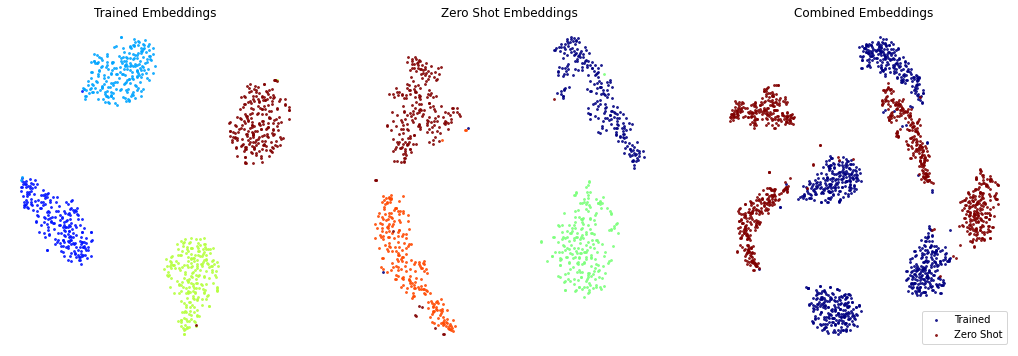
\includegraphics[width=0.9\textwidth]{../plots/final.png}
	\caption{t-SNE visualization of trained and zero shot embeddings}
\end{figure}


\chapter{Conclusion}

Embedding networks can be a very powerful tool for image classification tasks.
They are especially useful in circumstances where other softmax based models begin to struggle.
Their ability to be trained on datasets with very few samples per class is very useful in tasks where its hard or costly to create bigger datasets.
The possibility to perform good zero shot detections is also very useful, this trait also allows to add new classes to a already trained model without the need to retrain it.
This opens the possibility to create a generic embedding model, that is trained on a huge dataset and then is used in a detection task without finetuning the model for this new task.
\\
Another interesting use case is unsupervised learning of embeddings with the use of augmentation strategies.
This allows the use of unlabeled datasets but the performance of the resulting model will be worse than if the model was trained on the same labeled dataset.



\bibliography{refs}

\end{document}